%\section{A brief introduction}
\label{misc:hmc}

Hamiltonian Monte Carlo had its beginnings in statistical physics, with the \citeyear{duane1987hybrid} paper by \citeauthor{duane1987hybrid}, using what they called `Hybrid Monte Carlo' in lattice models of quantum theory.
Their work merged the approaches of molecular dynamics and Markov chain Monte Carlo methods.
As an interesting side note, their method abbreviates also to `HMC', but throughout the statistical literature, it is more commonly referred to by its more descriptive name Hamiltonian Monte Carlo.
Incidentally, the use of HMC started with applications to neural networks as early as 1996 (see \cite{neal2011mcmc} for an excellent review of the subject matter).
It was not until 2011 when active development of the method, and in particular, software for for statistical applications began.
The \proglang{Stan} initiative \citep{carpenter2016stan} began in response to difficulties faced when performing full Bayesian inference on multilevel generalised linear models.
These difficulties mainly involved poor efficiency in usual MCMC samplers, particularly due to high autocorrelations in the posterior chains, which meant that many chains and many iterations were required to get an adequate sample.
It was a case of exhausting all possible algorithmic remedies for existing samplers (Gibbs samplers, Metropolis samplers, etc.), and realising that fundamentally not much improvement can be had unless a novel sampling technique was discovered.

The basic idea behind HMC is to use Hamiltonian dynamics to propose new states in the posterior sampling, rather than relying on `random walks'.
If one were to understand and use the geometry of the posterior density to one's benefit, then it should be possible to generate new proposal states with high probabilities of acceptance and move far away from the current state.
Hamiltonian dynamics, like classical Newtonian mechanics, provides a framework for modelling the motion of a body in space across time $t$. 
Additionally, Hamiltonian dynamics concatenates the position vector $x$ with its momentum $z$, and the motion of $x$ in $d$-dimensional space is then described through Hamilton's equations
\begin{equation}\label{eq:hamilton1}
  \frac{\d x}{\d t} = \frac{\partial H}{\partial z}
  \hspace{0.5cm}\text{and}\hspace{0.5cm}
  \frac{\d z}{\d t} = -\frac{\partial H}{\partial x},
\end{equation}
where $H=H(x,z)$ is called the Hamiltonian of the system.
The Hamiltonian is an operator which encapsulates the total energy of the system.
In a closed system, one can express the sum of operators corresponding to the kinetic energy $K(p)$ and the potential energy $U(z)$ of the system
\begin{equation}\label{eq:hamilton2}
  H(x,z) = K(z) + U(x).
\end{equation}
Substituing \cref{eq:hamilton2} into \cref{eq:hamilton1}, we get the system of partial differential equations (PDEs)
\begin{equation}\label{eq:hamilton3}
  \frac{\d x}{\d t} = \frac{\partial}{\partial z} K(z)
  \hspace{0.5cm}\text{and}\hspace{0.5cm}
  \frac{\d z}{\d t} = -\frac{\partial}{\partial x}U(x).
\end{equation}

To describe the evolution of $\big(x(t),z(t)\big)$ from time $t$ to $t+T$, it is necessary to discretise time, and split $T = L\epsilon$.
The quantity $L$ is known as the number of \emph{leapfrogs}, and $\epsilon$ the \emph{step size}.
\begin{center}
  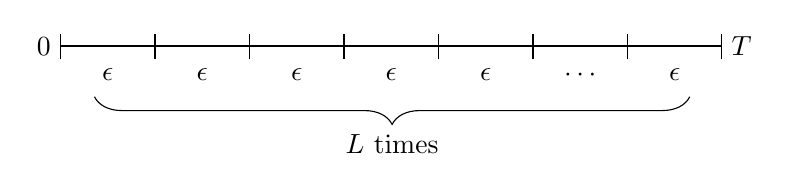
\begin{tikzpicture}[xscale=1.2, yscale=0.8]
    \draw [thick]  (0,0) -- (7,0);
    \foreach \x in  {0,1,2,3,4,5,6,7}
    \draw (\x,-.2) -- (\x, .2);
    \foreach \x in  {0.5,1.5,2.5,3.5,4.5}
    \node[align=center, below] at (\x,-.2) {$\epsilon$};
    \node[align=center, below] at (5.5,-.2) {$\cdots$};
    \node[align=center, below] at (6.5,-.2) {$\epsilon$};
    \node[align=center, left] at (0,0) {$0$};
    \node[align=center, right] at (7,0) {$T$};
    \draw[decorate, decoration={brace, mirror, amplitude=10pt}, xshift=-4pt, yshift=0pt]
    (0.5,-0.8) -- (6.8,-0.8) node [midway,below,yshift=-10pt] {$L$ times};
  \end{tikzpicture}
\end{center}
The system of PDEs is solved using Euler's method, or the more commonly used leapfrog integration, which is a three-step process:
\begin{table}[H]
  \centering
  \begin{tabular}{lrl}
    1. \textbf{Half-step momentum.} 
    &$z(t + \epsilon/2) =$ 
    &\hspace{-7pt}$z(t) - \frac{\epsilon}{2} \, \frac{\partial}{\partial x} U \big( x(t) \big)$ \\[0.6em]
    2. \textbf{Full-step position.} 
    &$x(t + \epsilon) =$ 
    &\hspace{-7pt}$x(t) + \epsilon \, \frac{\partial}{\partial  z} K \big(  z(t + \epsilon / 2) \big)$ \\[0.6em]
    3. \textbf{Half-step momentum.} 
    &$z(t + \epsilon) =$ 
    &\hspace{-7pt}$z(t + \epsilon/2) =  z(t) - \frac{\epsilon}{2} \, \frac{\partial}{\partial x} U \big( x(t) \big)$ \\[0.6em]
  \end{tabular}
\end{table}
\vspace{-1.5em}
\noindent in which steps 1--3 are repeated $L$ times.

Having knowing the formula for how particles move in space, we can use this information to treat random points drawn from some probability density as `particles'.
Randomness of position and momentum are prescribed through probability densities on each.
Given some energy function $E(\theta)$ over states $\theta$, the \emph{canonical distribution} of the states $\theta$ (otherwise known as the \emph{canonical ensemble}) is given by the probability density function
\[
  p(\theta) \propto \exp \left( -\frac{E(\theta)}{k\tau} \right),
\]
where $k$ is Boltzmann's constant, $\tau$ is the absolute temperature of the system.
The Hamiltonian is one such energy function over states $(x,z)$.
By replacing $E(\theta)$ by \cref{eq:hamilton2} in the pdf above, we realise that the distribution for $x$ and $z$ are independent.
The system can be manipulated such that $k\tau=1$---in any case, these are constants which can be absorbed into one of the terms in the pdf anyway.

Using a \emph{quadratic kinetic energy} function $K(z) = z^\top M^{-1} z/2$\footnotemark, we find that the probability density function for $z$ is
\[
  p(z) \propto \exp \left(-\half z^\top M^{-1} z \right),
\]
implying $z\sim\N_d(0,M)$.
Here, $M = \diag(m_1,\dots,m_d)$ is called the \emph{mass matrix}, which obviously serves as the variance for the randomly distributed $z$.
As for the potential energy, choose a function such that $U(x) = -\log p(x)$, implying $p(x) \propto \exp \big( -U(x) \big)$.
Here, $p(x)$ represents the target density from which we wish to sample, for instance, a posterior density of interest.
Thus, to sample variables $x$ from $p(x)$, one artificially introduces momentum variables $z$ and sample jointly instead from $p(x,z) = p(z)p(z)$, and discarding $z$ thereafter.
The HMC algorithm is summarised in \cref{alg:hmc}.

%\vspace{1em}
\algrenewcommand{\algorithmiccomment}[1]{{\color{gray} \hfill $\triangleright$ #1}}
\begin{algorithm}[hbt]
\caption{Hamiltonian Monte Carlo}
\label{alg:hmc}
\begin{algorithmic}[1]
  \State \textbf{initialise} $x^{(0)}$, $z^{(0)}$ and choose values for $L$, $\epsilon$ and $M$
  \For{$t=1,\dots,T$}
    \State Draw $z\sim\N_d(0,M)$ \Comment{Perturb momentum}
    \State Move $(x^{(t)},z^{(t)}) \mapsto (x^*,z^*)$ using Hamiltonian dynamics  \Comment{Proposal state}
    \State Accept/reject proposal state, i.e. \Comment{Metropolis update}
    \[
      (x^{(t+1)},z^{(t+1)}) \gets 
      \begin{cases}
        (x^*,z^*) & \text{w.p. } \min(1,A) \\
        (x^{(t)},z^{(t)}) & \text{otherwise}
      \end{cases}
    \]
    where
    \[
      A = \frac{p(x^*,z^*)}{(x^{(t)},z^{(t)})} = \exp\left( H(x,z) -  H(x^{(t)},z^{(t)}) \right)
    \]
  \EndFor
  \State \textbf{return} Samples $\big\{x^{(1)},\dots,x^{(T)}\big\}$
\end{algorithmic}
\end{algorithm}

\begin{figure}[p]
  \vspace{-10pt}
  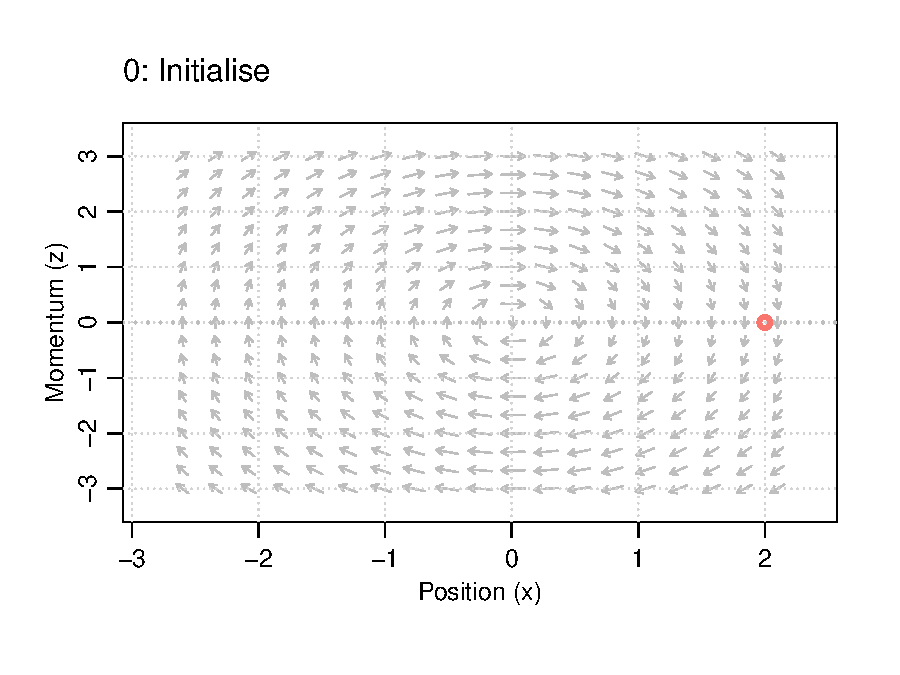
\includegraphics[width=0.49\textwidth]{figure/04-phase1}
  \vspace{-20pt}
  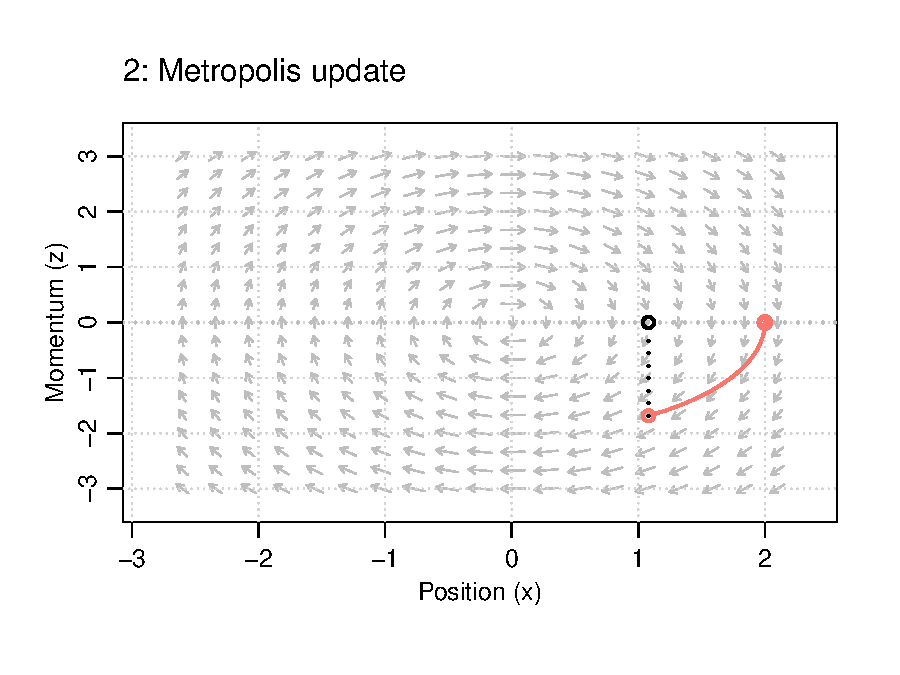
\includegraphics[width=0.49\textwidth]{figure/04-phase2}
  \vspace{-20pt}
  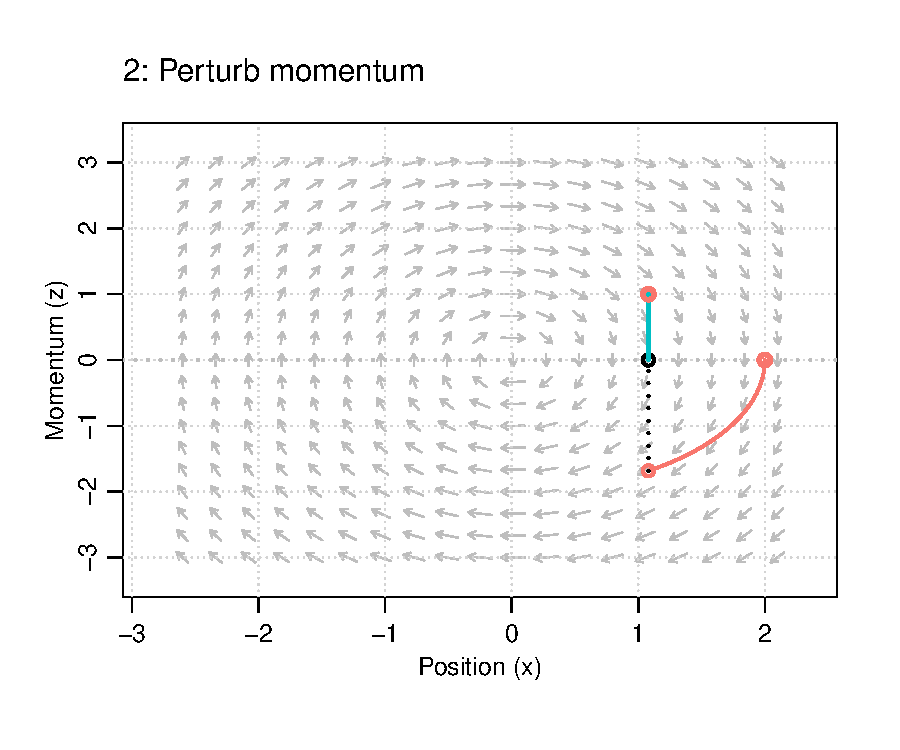
\includegraphics[width=0.49\textwidth]{figure/04-phase3}
  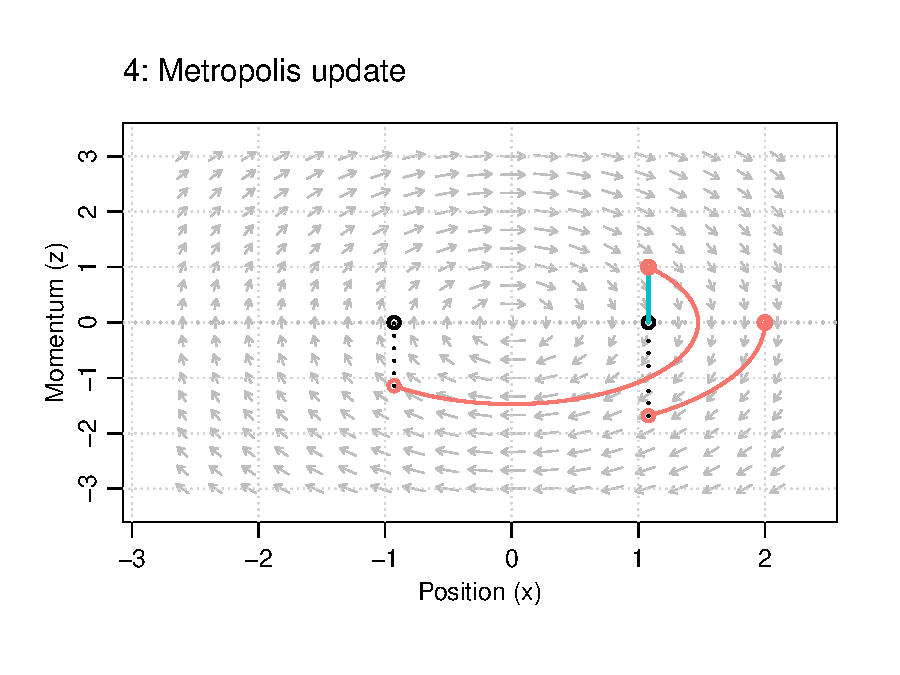
\includegraphics[width=0.49\textwidth]{figure/04-phase4}
  \vspace{-20pt}
  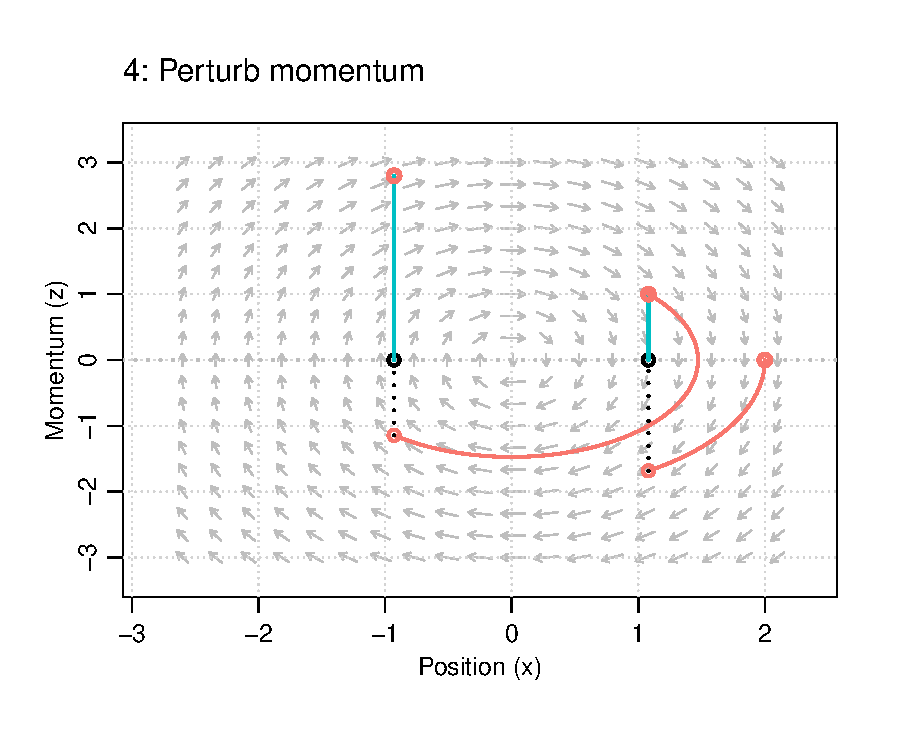
\includegraphics[width=0.49\textwidth]{figure/04-phase5}
  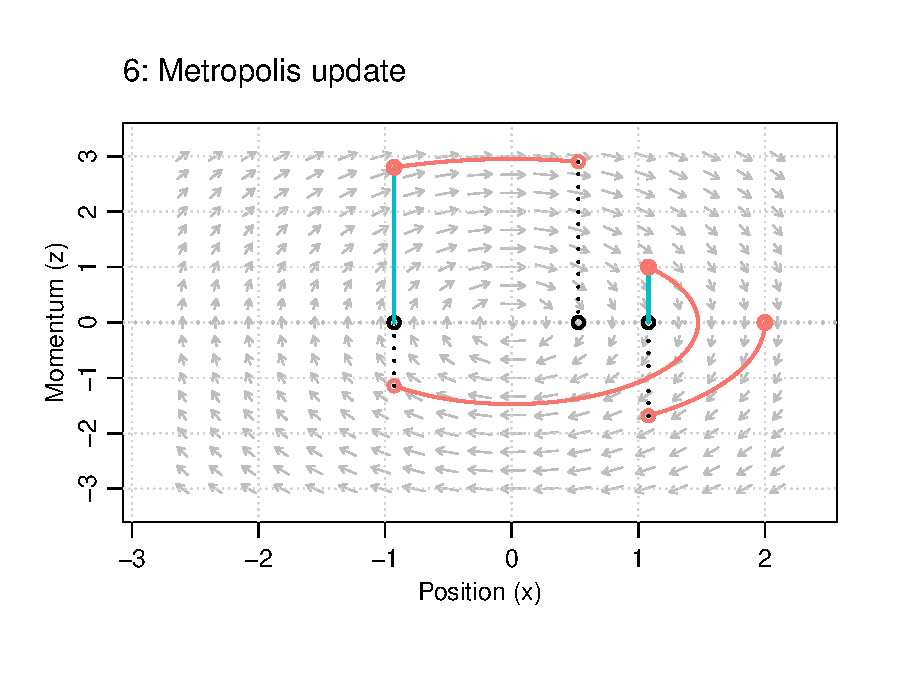
\includegraphics[width=0.49\textwidth]{figure/04-phase6}
  \vspace{-20pt}  
  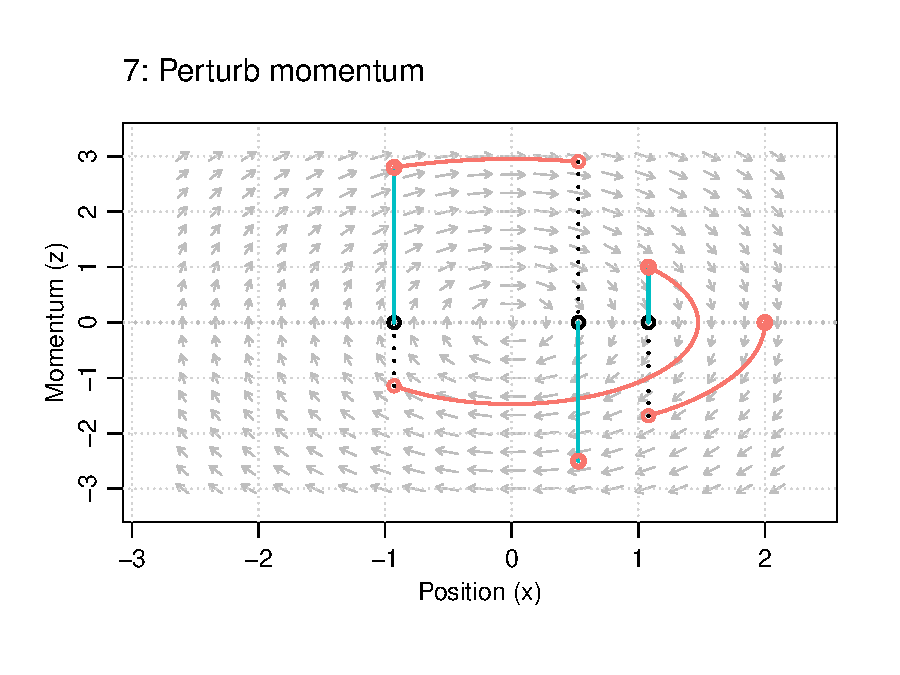
\includegraphics[width=0.49\textwidth]{figure/04-phase7}
  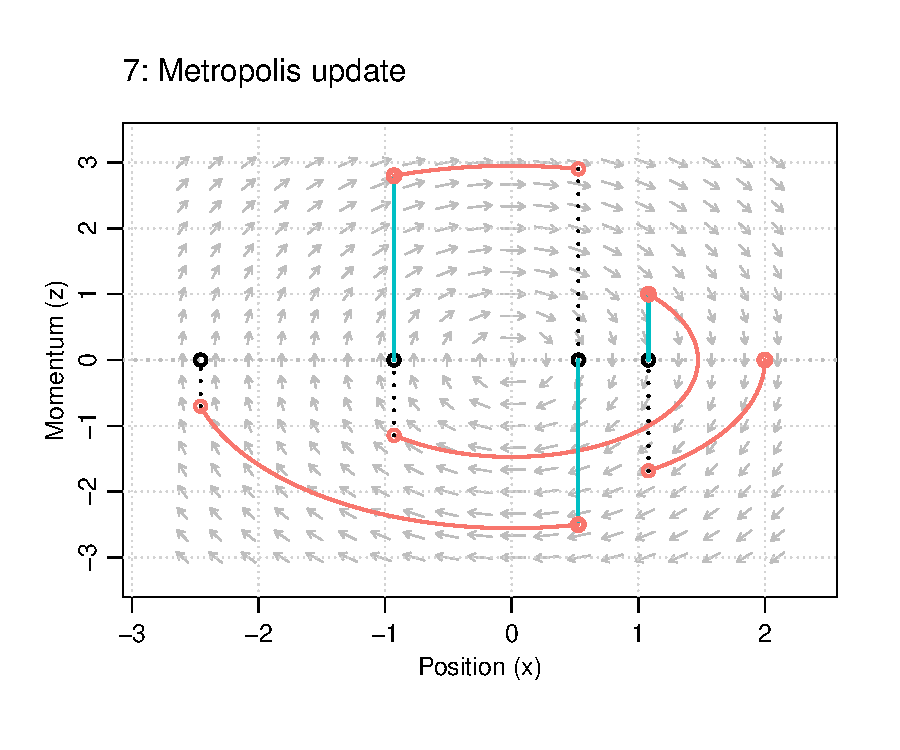
\includegraphics[width=0.49\textwidth]{figure/04-phase8}
  \caption{A phase diagram schematic of HMC sampling in one-dimension. At step 0, initialise values for momentum and position. At step 1, simulate movement using Hamiltonian dynamics, accept position and discard momentum. At step 2, perturb momentum using a normal density, then repeat.}
\end{figure}
\vspace{-0.5em}

HMC is often times superior to standard Gibbs sampling, for a variety of reasons. 
For one, conjugacy does not play any role in the efficiency of the HMC sampler, thus freeing the modeller to choose more appropriate and more intuitive prior densities for the parameters of the model. 
For another, the HMC sampler is designed to incite little autocorrelations between samples, and thus increasing efficiency.

Several drawbacks do exist with the HMC sampler. Firstly, it is impossible to directly sample from discrete distributions $p(x)$.
More concretely, HMC requires that the domain of $p(x)$ is continuous and that $\partial \log p(x) / \partial x$ is inexpensive to compute.
To work around this, one must reformulate the model by marginalising out the discrete variables, and obtain them back later by separately sampling from their posteriors.
Alternatively, a Gibbs sampler specifically for the discrete variables could be augmented with the HMC sampler.
The other drawback of HMC is that there are many tuning parameters (leapfrog $L$, step-size $\epsilon$, mass matrix $M$, etc.)  that is not immediately easy to perfect, at least not to the novice user. 

The implementation of HMC by the programming language \proglang{Stan}, which interfaces many other programming languages including \proglang{R}, \proglang{Python}, \proglang{MATLAB}, \proglang{Julia}, \proglang{Stata} and \proglang{Mathematica}, is a huge step forward in computational Bayesian analysis.
\proglang{Stan} takes the liberty of performing all the tuning necessary, and the practitioner is left with simply specifying the model. 
A vast library of differentiable probability functions are available, with the ability to bring your own code as well.
Development is very active and many improvements and optimisations have been made since its inception.

\footnotetext{Thinking back to elementary mechanics, this is the familiar $\half m v^2$ formula for kinetic energy and substituting in the identity $z =mv$, where $m$ is the mass of the object, and $v$ is its velocity.}